% !TeX program = xelatex
\documentclass[9pt]{beamer}
\usepackage{xcolor}
\definecolor{orange}{HTML}{FF1053}
\definecolor{lightgray}{HTML}{CCCCCC}
\definecolor{red}{HTML}{AC454A}
\definecolor{brown}{HTML}{EAD296}
\definecolor{darkgrey}{HTML}{313630}
\definecolor{cornflower}{HTML}{247BA0}
\definecolor{sienna}{HTML}{6C464F}
\usefonttheme{professionalfonts} % using non standard fonts for beamer
\usefonttheme{serif} % default family is serif
\usepackage{fontspec}
\usepackage{setspace}
\usepackage{natbib}
\usepackage{animate}
\usepackage{graphicx}
%\usepackage[T1]{fontenc}

\bibliographystyle{abbrv}
%\setmainfont{Liberation Serif}
%\setmainfont{Liberation Serif}
\setmainfont{Comfortaa}
%\usepackage[T1]{fontenc}

\setbeamercolor{frametitle}{bg=orange,fg=white}
\setbeamercolor{author in head/foot}{bg=orange,fg=white}

%\setbeamerfont{page number}{size=\Huge}

%\setbeamertemplate{itemize itemjpegs}[circle]
\useinnertheme{circles}
\setbeamercolor{palette primary}{bg=orange,fg=white}
%\setbeamercolor{palette secondary}{bg=red,fg=white}
\setbeamertemplate{itemize item}{\color{darkgrey}$\circ$}
\setbeamercolor{structure}{fg=darkgrey} % itemize, enumerate, etc

%\setbeamercolor{section in head/foot}{bg=red}
\setbeamercolor{title}{fg=orange} %, bg=brown
\setbeamercolor{author}{fg=darkgrey}
\setbeamercolor{institute}{fg=darkgrey}
\setbeamercolor{date}{fg=darkgrey}
%\setbeamercolor{normal text}{fg=darkgrey}
\makeatletter
\setbeamertemplate{headline}{%
	\usebeamercolor[bg]{frametitle}\rule{\textwidth}{1cm}
}
\setbeamerfont{title}{size=\LARGE}
\setbeamerfont{institute}{size=\normalsize}
\renewcommand*{\bibfont}{\scriptsize}


\setbeamertemplate{frametitle}{%
	\vskip-1cm%
	\begin{minipage}[c][\headheight][c]{\textwidth}%
		\usebeamerfont{frametitle}
		\strut\insertframetitle\par
		{%
			\ifx\insertframesubtitle\@empty%
			\else%
			{\usebeamerfont{framesubtitle}\usebeamercolor[fg]{framesubtitle}\strut\insertframesubtitle\par}%
			\fi
		}%      
		\vspace*{0.05cm}
	\end{minipage}%
	\vskip-0.1em
}
%\setbeamertemplate{footline}{%
%	\leavevmode%
%	\hbox{\begin{beamercolorbox}[wd=\paperwidth,ht=4.5ex,dp=3.125ex]{author in head/foot}%
%			\usebeamerfont{author in head/foot} bar
%	\end{beamercolorbox}}%
%	\vskip0pt%
%}
\makeatother


\title{Simulation-based Inference \\
	\small Inverting Simulators}
\author{Talk by Stefan Wezel}
\institute{mlcolab @ Tübingen University Cluster of Excellence}
\date{\today}


%\setbeamertemplate{sidebar right}{}
%\setbeamertemplate{footline}{%
%	\hfill\usebeamertemplate***{navigation symbols}
%	\hspace{1cm}\insertframenumber{}}
\setbeamerfont{page number in head/foot}{size=\small}
    \setbeamertemplate{footline}{%
	\raisebox{5pt}{\makebox[\paperwidth]{\hfill\makebox[10pt]{\scriptsize\insertframenumber}}}}
\setbeamertemplate{navigation symbols}{}
%\onehalfspacing
\setstretch{1.3}
\begin{document}
	

\setbeamercolor{background canvas}{bg=white}
\setbeamercolor{normal text}{fg=darkgrey}
\usebeamercolor[fg]{normal text}
\begin{frame}[plain]
	\titlepage
\end{frame} 



\setbeamercolor{background canvas}{bg=white}
\setbeamercolor{normal text}{fg=darkgrey}
\usebeamercolor[fg]{normal text}
\setbeamertemplate{itemize item}{\color{darkgrey}$\circ$}
\begin{frame}
\frametitle{Overview}
\framesubtitle{}
\begin{itemize}
	\item The problem setting %(as this is rather unfamiliar to ML researchers)
	\item Traditional approaches and their issues
	\item Using Bayesian Neural Nets to alleviate them
	\item A worked example
	\item A more interesting, real-world example
	\item Outlook %(and some advertisement)
\end{itemize}
\end{frame} 






\begin{frame}
\frametitle{What and Why?}
\framesubtitle{An Example}
\begin{itemize}
	\item Imagine you are a astronomer
	\item You observe planetary movements
	\item and find that two parameters determine the movement (mass and velocity) (and some noise)
	\item So you build a mechanistic model that can simulate observations
	\item But what do we actually care about?
	\begin{itemize}
		\item What was the mass and velocity of that planet
%		\item In other words: what were the parameters $\theta$ for observation $x_0$
	\end{itemize}
%	\item You're simulator has no direct answer to this question except for trying everything out
\end{itemize}
\end{frame} 


\begin{frame}
\frametitle{What and Why?}
\framesubtitle{Formalizing our Example}
\begin{itemize}
	\item Mechanistic model (simulator) has parameters $\theta$ and produces data $\hat{x}$
	\begin{itemize}
		\item It implicitly defines $p(\hat{x}|\theta)$ (it yields samples from this distribution)
	\end{itemize}
	\item Given a (real) observation $x_0$, we would be interested in the parameters that produced it
	\begin{itemize}
		\item $p(\theta|x_0)$ -> posterior over parameters
		\item In simple cases, we could apply Bayes' rule and compute it analytically
		\item What is simple? If we know Likelihood
		\item But often we would not
	\end{itemize}
\end{itemize}
\end{frame} 



\begin{frame}
\frametitle{What and Why?}
\framesubtitle{Simulation-based Inference to the rescue}
\begin{itemize}
		\item This is exactly a problem setting that scientists often deal with
	\begin{itemize}
		\item They have a sophistic model (the simulator) that encapsulates a lot of prior knowledge
		\item But inference in this setting often boils down to: What were parameters that produced this observation
	\end{itemize}
	\item Simulation-based Inference inference tries to solve this problem
	\item by inverting the simulator
\end{itemize}
\end{frame} 




\begin{frame}
\frametitle{Simulation-based Inference}
\framesubtitle{Traditional Approach}
\begin{itemize}
	\item Broader term: Approximate Bayesian Computation (ABC)
	\begin{itemize}
		\item Rejection ABC
		\item Sampling ABC (perturbe intitial params)
		\item Sequential ABC
	\end{itemize}
	\begin{itemize}
		\item But gives only point estimates, not full posterior
		\item within $\epsilon$
	\end{itemize}	
\end{itemize}
\end{frame} 




\begin{frame}
\frametitle{Learning a Posterior}
\framesubtitle{Bayesian Neural Nets to the Rescue}
\begin{itemize}
	\item Create $n$ training samples
	\item learn posterior over parameters by parametrizing GMM with DNN
\end{itemize}
\end{frame} 




\begin{frame}
\frametitle{How to use SBI?}
\framesubtitle{Some advertisement}
\begin{itemize}
	\item Now that you are pretty excited about SBI and its applications
	\item mlcolab and mackelab is developing a python (and eventually Julia) library (that I've used earlier)
	\item If you are interested: try it out and give us your feedback
	\item link to colab
	\item link to github
		\begin{figure}
		\flushleft
		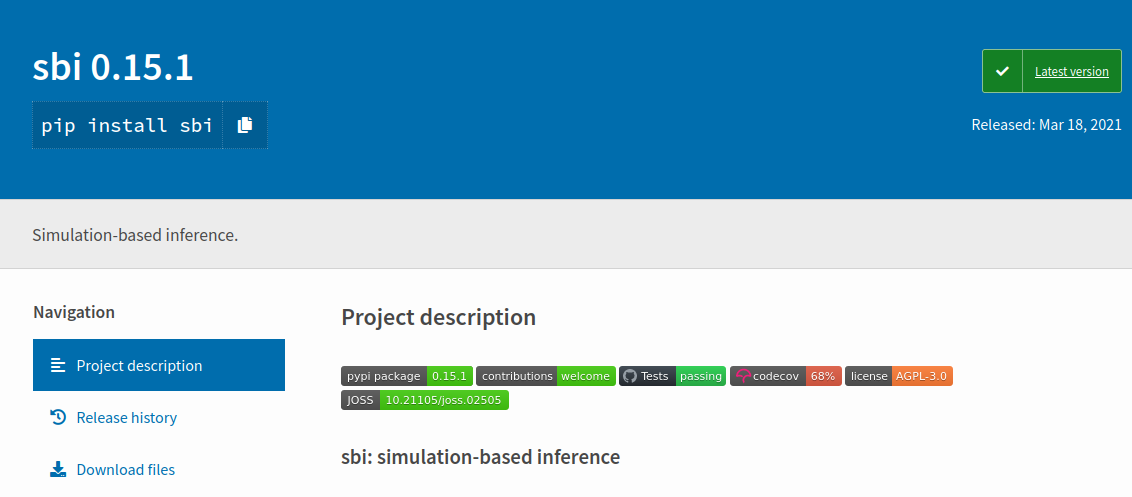
\includegraphics[width=.75\linewidth]{figures/sbipypi.png}
	\end{figure}
\end{itemize}
\end{frame} 






\begin{frame}
\frametitle{}
\framesubtitle{}
\begin{itemize}
	\item 
\end{itemize}
\end{frame} 



\begin{frame}
\frametitle{How}
\framesubtitle{Approximate Bayesian Computation}
\begin{itemize}
	\item Finding parameters/posterior over parameters with
	\begin{itemize}
		\item Rejection ABC
		\item Markov Chain Monte Carlo ABC
		\item Sequential Monte Carlo ABC
		\item ...
	\end{itemize}
	\item Problems
	\begin{itemize}
		\item 
	\end{itemize}
\end{itemize}
\end{frame} 



\begin{frame}
\frametitle{What}
\framesubtitle{is Simulation-based Inference?}
\begin{itemize}
	\item If we know generating factors, we can build a simulator
	\item But we want to constrain simulator output on observations from real world
	\item Thus we need realistic values for simulator parameters
	\item -> inverse problem
	\item SBI solvers this inverse problem using Bayesian inference
\end{itemize}
\end{frame} 


\begin{frame}
\frametitle{How}
\framesubtitle{does Simulation-based Inference work?}
\begin{figure}
	%	\flushright
	%	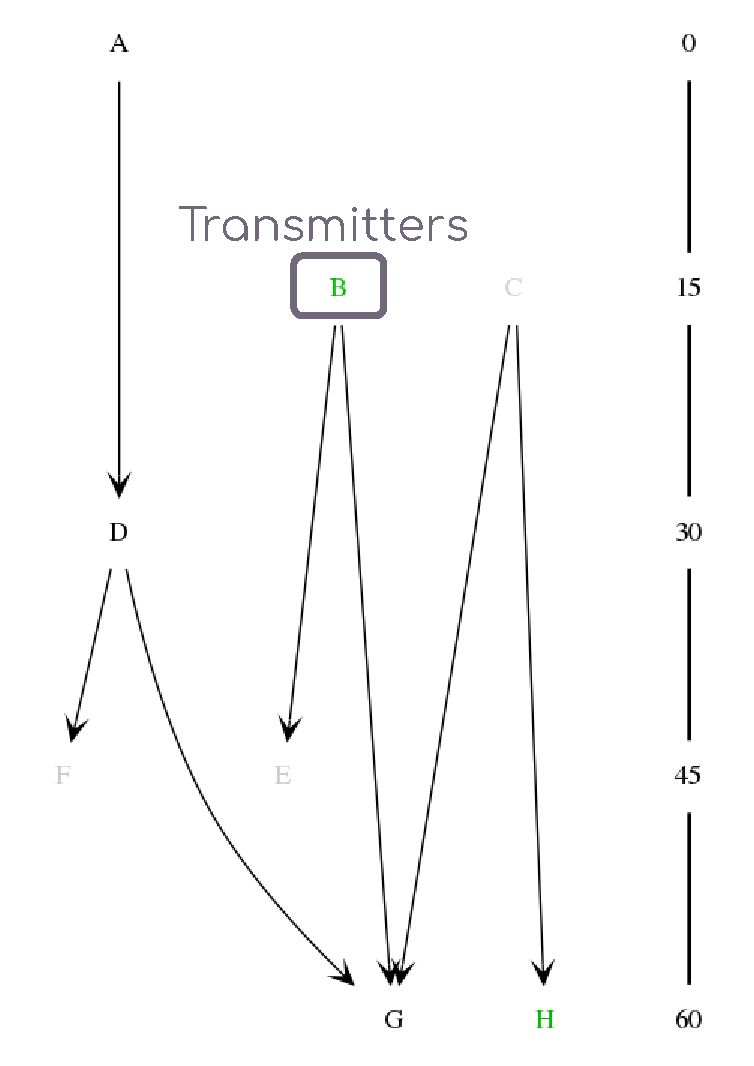
\includegraphics[width=.5\linewidth]{figures/isnalyser_parts_1.pdf}
\end{figure}
\end{frame} 



\end{document}


